\chapter{Y00-量子暗号の信号状態
}
まず、コヒーレント状態について説明する。コヒーレント状態は、複素振幅$\alpha=x+iy$を持つ理想的なレーザー光を表す量子状態である。コヒーレント状態の複素振幅$\alpha$は複素平面上で平均$(x,y)^T$、共分散行列 
$$
\begin{pmatrix}
1/4&0\\
0&1/4
\end{pmatrix}
$$
の正規分布に従って揺らいでいる.\figref{Fig:3_1}は、平均$(x,y)^T$のコヒーレント状態の揺らぎを表している。

\begin{figure}[htbp]
        \centering   
        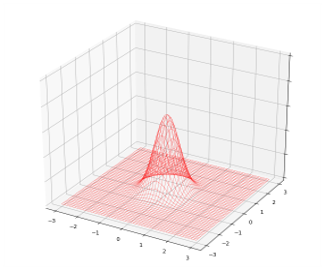
\includegraphics[width=0.7\textwidth]{img/zemi1.png}
        \caption[sample image (png)]{コヒーレント状態のゆらぎ}
        \label{Fig:3_1}
    \end{figure}


Y00-量子暗号の信号状態について説明する。青い丸がコヒーレント状態でこれを使って通信を行う。使用する基底によって0と1に対応する信号状態が異なる。例えば基底1を使って0を送りたいときは0のコヒーレント状態を使い、1を送りたいときは0のコヒーレント状態を使う。正規の受信者と送信者はどの基底を使って通信をしているのかわかる。同じ基底のコヒーレント状態は離れているので盗聴されにくいため、安全性が保証される。$S_{max}$は信号の最大強度を表している.$B$個の規定で通信する場合間隔の個数が$2B-1$個となることから隣接信号間の間隔は$S_{max}/2B-1$になる。このことから基底$k$の信号状態は

$$
\left |\frac{S_{max}}{2B-1}\right\rangle,\left |\frac{S_{max}}{2B-1}(B+k)\right\rangle
$$

\begin{figure}[htbp]
        \centering   
        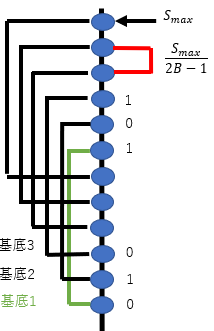
\includegraphics[width=0.5\textwidth]{img/zemi2.png}
        \caption[sample image (png)]{量子暗号の信号状態.}
        \label{Fig:3_2}
    \end{figure}
